% Copyright 2019 Clara Eleonore Pavillet

% Author: Clara Eleonore Pavillet (original author), Leonard Quentin Marcq (modified for Tsinghua), 赵宗义 (参与了修改)
% Description: This is an unofficial Tsinghua University Beamer Template I made from scratch. Feel free to use it, modify it, share it.
% Version: 1.1


\documentclass{beamer}
\usepackage{ctex}
\usepackage{fontspec}
% Load Packages
\usepackage[utf8]{inputenc}
\usepackage{xcolor}
\usepackage{tikz}
\usetikzlibrary{positioning,calc}
\usepackage{graphicx}
\usepackage{hyperref}
\usepackage{amsmath}
\usepackage{listings}
%\usepackage{fontawesome}

% Define Commands
\newcommand*{\ClipSep}{0.06cm} %To adjust footer logo
\newcommand{\E}{\mathrm{e}\,} %\def\I{e} % used to defined e for exp(x), see later what it should be
\newcommand{\ud}{\mathrm{d}}
\lstset{numbers=left, numberstyle=\tiny, stepnumber=1,firstnumber=1,breaklines=true,
    numbersep=5pt,language=Python,
    stringstyle=\ttfamily,
    basicstyle=\footnotesize, 
    showstringspaces=false
}

\usetheme{tsinghua}

\usepackage{amsmath,amssymb,amsthm,srcltx}
\usepackage{mathtools}
%\usepackage[dvips]{color}
%\usepackage[margin]{fixme}
%\usepackage{enumerate}
\usepackage{stmaryrd}
%\usepackage[colorinlistoftodos]{todonotes}
%\usepackage{bbm}
%\usepackage{dsfont}
%\numberwithin{equation}{section}
%\usepackage{fullpage}

%%%<<<---
\newcommand{\system}{HashFlow}
\newcommand{\variable}{\mathrm}
\newcommand{\field}{\mathsf}
%%%--->>>

\def\dbB{\mathbb{B}}
\def\dbC{\mathbb{C}}
\def\dbD{\mathbb{D}}
\def\dbE{\mathbb{E}}
\def\dbF{\mathbb{F}}
\def\dbG{\mathbb{G}}
\def\dbH{\mathbb{H}}
\def\dbI{\mathbb{I}}
\def\dbJ{\mathbb{J}}
\def\dbK{\mathbb{K}}
\def\dbL{\mathbb{L}}
\def\dbM{\mathbb{M}}
\def\dbN{\mathbb{N}}
\def\dbP{\mathbb{P}}
\def\dbR{\mathbb{R}}
\def\dbU{\mathbb{U}}
\def\dbS{\mathbb{S}}
\def\dbT{\mathbb{T}}
\def\dbQ{\mathbb{Q}}
\def\dbY{\mathbb{Y}}


\newcommand{\cB}{\mathcal{B}}
\newcommand{\cC}{\mathcal{C}}
\newcommand{\cD}{\mathcal{D}}
\newcommand{\cE}{\mathcal{E}}
\newcommand{\cF}{\mathcal{F}}
\newcommand{\cG}{\mathcal{G}}
\newcommand{\cH}{\mathcal{H}}
\newcommand{\cI}{\mathcal{I}}
\newcommand{\cK}{\mathcal{K}}
\newcommand{\cL}{\mathcal{L}}
\newcommand{\cM}{\mathcal{M}}
\newcommand{\cN}{\mathcal{N}}
\newcommand{\cP}{\mathcal{P}}
\newcommand{\cQ}{\mathcal{Q}}
\newcommand{\cR}{\mathcal{R}}
\newcommand{\cS}{\mathcal{S}}
\newcommand{\cT}{\mathcal{T}}
\newcommand{\cU}{\mathcal{U}}
\newcommand{\cV}{\mathcal{V}}
\newcommand{\cX}{\mathcal{X}}
\newcommand{\cY}{\mathcal{Y}}
\newcommand{\cZ}{\mathcal{Z}}

\newcommand{\Cbf}{\mathbf{C}}
\newcommand{\frakC}{\mathfrak{C}}

\def\no{\noindent}
\def\eq{\eqalign}
\def\ss{\smallskip}
\def\ms{\medskip}
\def\bs{\bigskip}
\def\q{\quad}
\def\qq{\qquad}
\def\hb{\hbox}
\def\pa{\partial}
\def\cd{\cdot}
\def\cds{\cdots}
%\def\lan{\langle}
\def\ran{\rangle}
\def\td{\nabla}



\def\a{\alpha}
\def\b{\beta}
\def\d{\delta}
\def\e{\varepsilon}
\def\Om{\Omega}
\def\om{\omega}
%\def\l{\lambda}
\def\L{\Lambda}
\def\t {\tau}
\def\si {\sigma}
\def\th {\theta}
\def\Th{\Theta}
\def\we {\wedge}
\def\eps{\varepsilon}





\newcommand{\ba}{\begin{array}} %%%MR : togliere gli array
\newcommand{\ea}{\end{array}}
\newcommand{\be}{\begin{equation}}
\newcommand{\ee}{\end{equation}}
\newcommand{\bea}{\begin{eqnarray}}
\newcommand{\eea}{\end{eqnarray}}
\newcommand{\beaa}{\begin{eqnarray*}}
\newcommand{\eeaa}{\end{eqnarray*}}


\newcommand{\Ind}{\mathbf{1}}

\DeclareMathOperator\sgn{\mathrm{sgn}}


\newcommand\ofp{\Omega,\mathcal{F},\mathbb{P}}

\newcommand{\sint}{\stackrel{\mbox{\tiny$\bullet$}}{}}
\newcommand\lan[1]{\langle #1 \rangle}
\newcommand\hvarphi{\hat{\varphi}}
\newcommand{\Var}{\operatorname{Var}} 
\newcommand{\diag}{\operatorname{diag}} 
\newcommand{\TV}{\operatorname{TV}}
\DeclareMathOperator{\conv}{conv}
\DeclarePairedDelimiter\abs{\lvert}{\rvert}
\let\brack\undefined
\DeclarePairedDelimiter\brack\lbrack\rbrack
\DeclarePairedDelimiter\paren{(}{)}
\DeclarePairedDelimiter\interinteg{[\![}{[\![}
\DeclarePairedDelimiter\ceil{\lceil}{\rceil}
\DeclareMathOperator\Cov{Cov}
\DeclareMathOperator*{\esssup}{ess\,sup}
\DeclareMathOperator*{\essinf}{ess\,inf}

%\newtheorem{theorem}{Theorem}[section] 
%\newtheorem{assumption}[theorem]{Assumption}
%\newtheorem{axiom}[theorem]{Axiom}
%\newtheorem{claim}[theorem]{Claim}
%\newtheorem{corollary}[theorem]{Corollary}
%\newtheorem{declaration}[theorem]{Declaration}
%\newtheorem{definition}[theorem]{Definition}
%\newtheorem{lemma}[theorem]{Lemma}
%\newtheorem{proposition}[theorem]{Proposition}
%\newtheorem{scholium}[theorem]{Scholium}
%\newtheorem{sublemma}[theorem]{Sublemma}
%\newtheorem{facts}[theorem]{Facts}

%\theoremstyle{definition}
%\newtheorem{example}[theorem]{Example}
%\newtheorem{remark}[theorem]{Remark}

\title{Machine Learning: Introduction}
%\titlegraphic{
\includegraphics[width=2cm]{Theme/Logos/sjtu_emblem_dark.png}}
\author{Yiqing LIN\ (林一青)\\[6pt]
Department of Statistics\\
School of Mathematical Sciences\\[6pt]
 (yiqing.lin@sjtu.edu.cn)\\[24pt]
%\institute{
\includegraphics[width=2cm]{Theme/Logos/sjtu_emblem_dark.png}\\[3pt]
Shanghai\ $\cdot$\ China\\[3pt]Dec. 16,\ 2020}
\date{} %\today

\begin{document}

{\setbeamertemplate{footline}{} 
\frame{\titlepage}}



%\begin{frame}{About Yiqing LIN}
%\textbf{Education background}
%\begin{itemize}
%\item 2003 B.S., Peking University (CHN)
%\item 2009 Qualification, Shandong University (CHN)
%\item 2013 Ph. D. Universit\'e de Rennes 1 (FRA)
%\end{itemize}
%\vspace{6pt}
%\textbf{Working experiences}
%\begin{itemize}
%\item 2013 - 2015, RA, Universit\"at Wien (AUT)
%\item 2015 - 2017, RA, \'Ecole Polytechnique (FRA)
%\item 2018 - \ \ \ \ \ \ , AP, Shanghai Jiao Tong University (CHN)
%\end{itemize}
%\end{frame}


\begin{frame}{Machine can learn}
\textbf{Computers do what they are told to do?}
\begin{itemize}
\item What the programmer know how to do
\item What can explain to the computers
\end{itemize}
\vspace{6pt}
\textbf{Programmed machine-learning system}
\begin{itemize}
\item Samuel ARTHUR, IBM, 1950s
\item Transistors may blow up
\item Test at the end of the assembly line
\end{itemize}
\end{frame}

\begin{frame}{Machine can learn}
\textbf{Checker player}
\begin{itemize}
\item The computer plays against Samuel (Testing job)
\item Having the computer learn how to play checkers
\begin{itemize}
\item Samuel teaches the computer to evaluate the costs and benefits of those moves (slow)
\item Samuel let one computer play another and take him out of the loop (fast)
\end{itemize}
\item The computer can easily beat Samuel consistently
\end{itemize}
\vspace{6pt}
\textbf{Amazing!!! The computer became a better checker player than its programmer!}
\end{frame}

\begin{frame}{Machine can learn}
\textbf{Task told by Samuel}
\begin{itemize}
\item Play checkers (No)
\item Learn-to-play-checkers-task (Yes)
\item {\it Deep blue, AlphaGo, etc...}
\end{itemize}
\vspace{6pt}
\textbf{Meta level task}
\begin{itemize}
\item A sentence refers to itself: {\it This sentence has five words.}
\item A task to develop skill at another task -- meta task 
\item Step outside the box and get the entirely new perspective on the world
\end{itemize}
\vspace{6pt}
\textbf{Conclusion:} Computers do what they are told, but they can be told to develop a capacity -- to LEARN.
\end{frame}


\begin{frame}{Machine learning}
\textbf{Machine learning}
\begin{itemize}
\item The academic field to study the computational learning systems
\item Learning from {\it examples}
\end{itemize}
\textbf{Catagory}
\begin{itemize}
\item Supervised learning
\item Unsupervised learning
\item Semi-supervised learning
\item Reinforcement learning (Deep learning?)
\end{itemize}
\end{frame}

\begin{frame}{Machine learning}
\textbf{Learning from examples}
\begin{itemize}
\item Cat or Dog? 
\item Each example is measured on a common group of attributes
\item Record the values for each attribute on each example
\end{itemize}
\begin{figure}
\centering
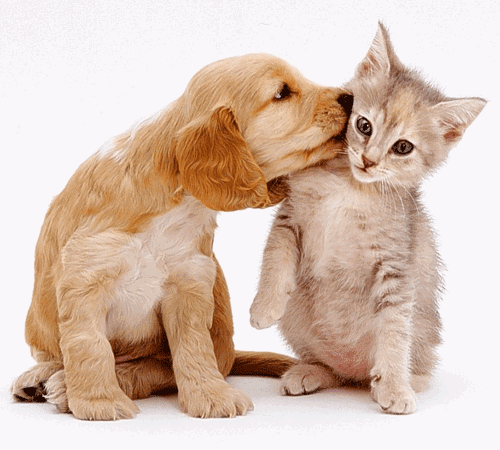
\includegraphics[width=4.2cm]{ep2.png}
\end{figure}
\end{frame}

\begin{frame}{Features}
\textbf{Features}
\begin{itemize}
\item What is measured -- attribute
\item What is the value -- value
\item What is the measured value -- feature
\end{itemize}
\begin{figure}
\centering
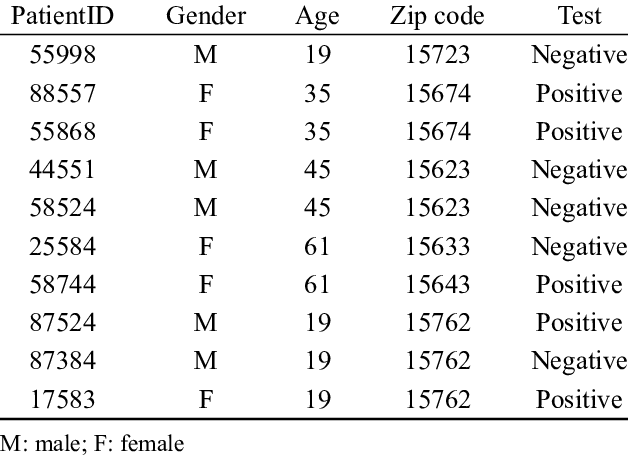
\includegraphics[width=5.6cm]{ep3.png}
\end{figure}
\end{frame}

\begin{frame}{Features}
\textbf{Types of values}
\begin{itemize}
\item Recorded as catalogues 
\begin{itemize}
\item $sex = \{ male, \ female\}$
\item $ethnic = \{african,\ asian, \ european,\ etc...\}$
\item discrete numbers, one value for each option or "true" vs "false"
\item Not meaningful in arithmetic performance 
\end{itemize}
\item Recorded as numbers
\begin{itemize}
\item Height, weight
\item Number of wheels on a car
\item continuous numbers
\item meaningful in arithmetic performance
\end{itemize}
\end{itemize}
\end{frame}

\begin{frame}{Target values and prediction}
\textbf{Problem: a patient developing cardiovascular heart}
\begin{itemize}
\item Target: Assessing the likelihood of a patient developing cardiovascular heart
\item Biomedical data from a health care provider
\item Label: did these folks develop heart disease?
\end{itemize}
\vspace{6pt}
\textbf{Possible target values}
\begin{itemize}
\item Develop any heart disease within ten years: yes/no
\item Develop $X$-level severity heart disease within ten years: None/I/II/III
\item Percent of coronary artery blokage
\end{itemize}
\vspace{6pt}
\textbf{Question: Ten years to wait???}
\end{frame}

\begin{frame}{Target values and prediction}
\textbf{Prediction}
\begin{itemize}
\item Predictive relationship: attributes today v.s. outcomes $Y$ years from now
\item Medical knowledge may help to reduce $Y$: percent of blockage is a critical amount
\end{itemize}
\vspace{6pt}
\textbf{Target features}
\begin{itemize}
\item Classification : $\{sick,\ healthy\}$ and $\{none,\ I,\ II, \ III\}$, categories
\item Regression: $0.55$, decimal numbers
\item Features: predictive / input features v.s. target features 
\end{itemize}
\end{frame}

\begin{frame}{Factory machines v.s. learning machines}
\textbf{A factory machine}
\begin{itemize}
\item Task: packaging
\item Run by the operator
\item Controlled by knobs
\item Left trays: matrials
\item Right trays: products
\end{itemize}
\begin{figure}
\centering
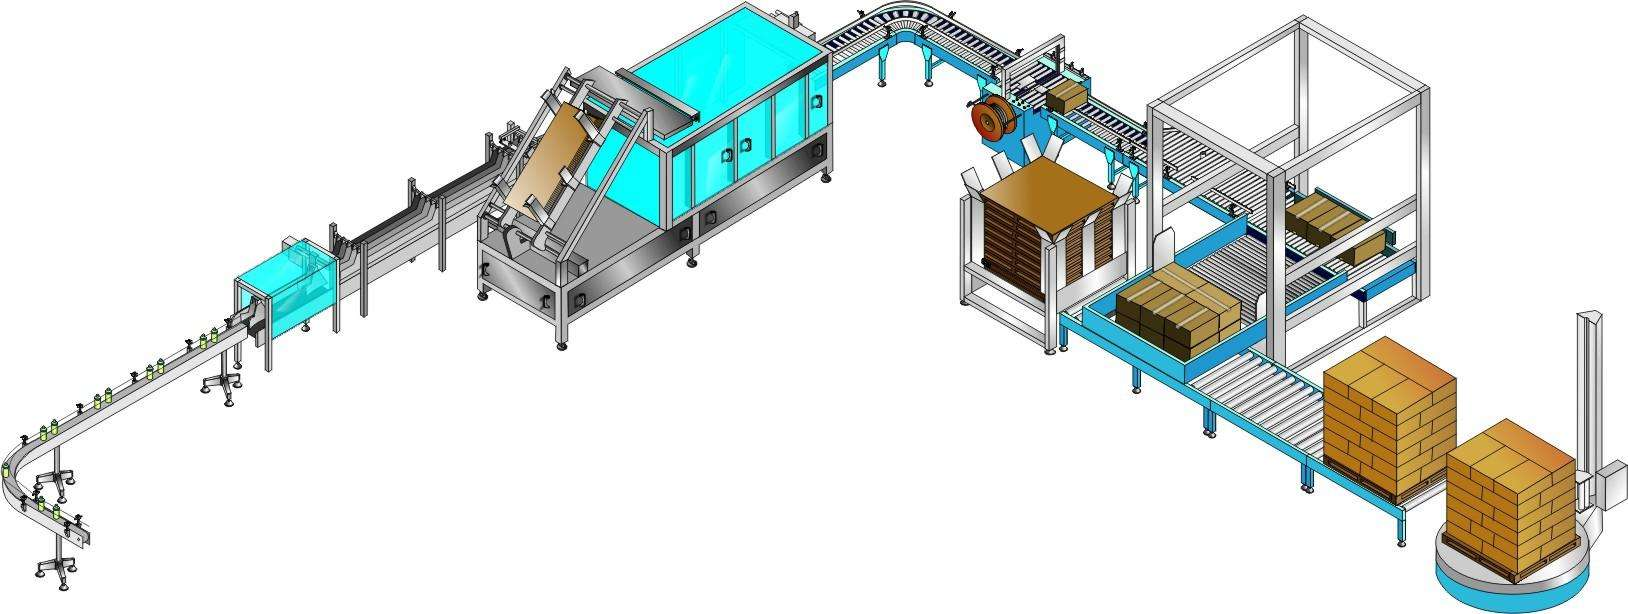
\includegraphics[width=8cm]{ep4.jpeg}
\end{figure}
\end{frame}

\begin{frame}{Factory machines v.s. learning machines}
\textbf{A learning machine}
\begin{itemize}
\item Task: producing a label
\item Run by the programmer
\item Controlled by parameters
\item Inputs: predictive features, $\{0, 1\}$ or $\{3.25, 3.34, 3.67\}$
\item Outputs: $\{cat, dog\}$
\end{itemize}
\vspace{6pt}
Learning algorithms are formal rules for how to use a well-defined method (implemented with a programming language) to set the knobs to good values.\\[6pt]
Learning machine is named as learning model, or for short, a model.
\end{frame}

\begin{frame}{Factory machines v.s. learning machines}
\textbf{Good values of the knobs}
\begin{itemize}
\item Compare predicted outcomes with known outcomes
\item Turn the knobs
\item Add a knob
\end{itemize}
\vspace{6pt}
\textbf{Knob-based learning methods}
\begin{itemize}
\item What knobs are there?
\item How do the knobs interact with an input of example
\item How do we set the knobs from some known data
\end{itemize}
\end{frame}

\begin{frame}{Examples: Predicting categories}
\begin{columns}
\column{0.75\textwidth}
\textbf{Problem}
\begin{itemize}
\item Handwritten ZIP codes on envelopes from U.S. postal mail
\item $16*16$ eight-bit grayscale maps
\item Predicting from the $16*16$ matrix of pixel intensities the identity $0, 1, 2, \ldots, 9$
\end{itemize}
\vspace{6pt}
\textbf{Challenge}
\begin{itemize}
\item The handwritten digit might be centred or cut-off on the edges
\item The handwritten digit might be blocked by lattices
\end{itemize}
\column{0.25\textwidth}
\begin{figure}
\centering
% Requires \usepackage{graphicx}
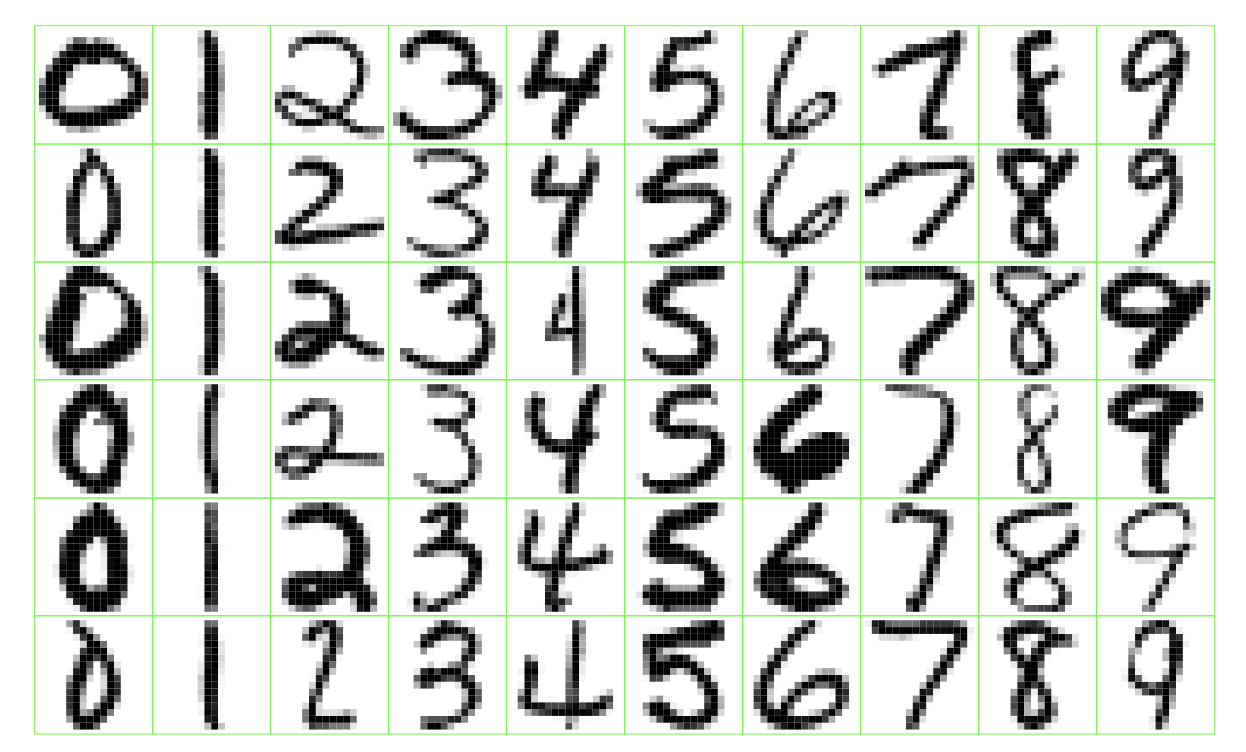
\includegraphics[width=3cm]{ep5.png}\\
{\tiny Handwritten digit recognition}
\end{figure}
\end{columns}

\end{frame}

\begin{frame}{Examples: Predicting categories}
\begin{columns}
\column{0.75\textwidth}
\textbf{Problem}
\begin{itemize}
\item Volatility daily prediction (VIX index on S\&P500) from 2014 to 2015
\item Predictors: word-stems occurrence count in {\it The New York Times} headlines of the last day
\item Predicting the direction of movement of the VIX index today
\end{itemize}
\vspace{6pt}
\textbf{Challenge}
\begin{itemize}
\item More than 47K stem-words (predictors)
\item A reasonable model?
\end{itemize}
\column{0.25\textwidth}
\begin{figure}
\centering
% Requires \usepackage{graphicx}
\includegraphics[width=3cm]{ep1.png}
{\tiny VIX index action}
\end{figure}
\end{columns}
\end{frame}

\begin{frame}{Examples: Predicting categories}
\begin{columns}
\column{0.75\textwidth}
\textbf{Problem}
\begin{itemize}
\item Patients' medical records, notes and medical images
\item Medical diagnosis: sick or healthy, disease 
\end{itemize}
\vspace{6pt}
\textbf{Challenge}
\begin{itemize}
\item Depending on information not captured in the records (eg. travel to tropical areas v.s. nasty diseases)
\item Different symptoms may link to different diagnoses, however, different diseases have common symptoms
\end{itemize}
\column{0.25\textwidth}
\begin{figure}
\centering
% Requires \usepackage{graphicx}
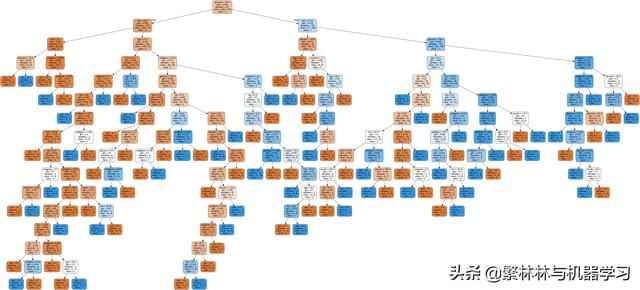
\includegraphics[width=3cm]{ep6.jpeg}
{\tiny Medical diagnosis}
\end{figure}
\end{columns}
\end{frame}

\begin{frame}{Examples: Predicting values}
\begin{columns}
\column{0.75\textwidth}
\textbf{Problem}
\begin{itemize}
\item Historical weather and corn yield data
\item Predicting future corn yield from new temperature observation 
\end{itemize}
\vspace{6pt}
\textbf{Challenge}
\begin{itemize}
\item Extreme weather and outliers
\item Randomness of the influence from other features 
\end{itemize}
\column{0.25\textwidth}
\begin{figure}
\centering
% Requires \usepackage{graphicx}
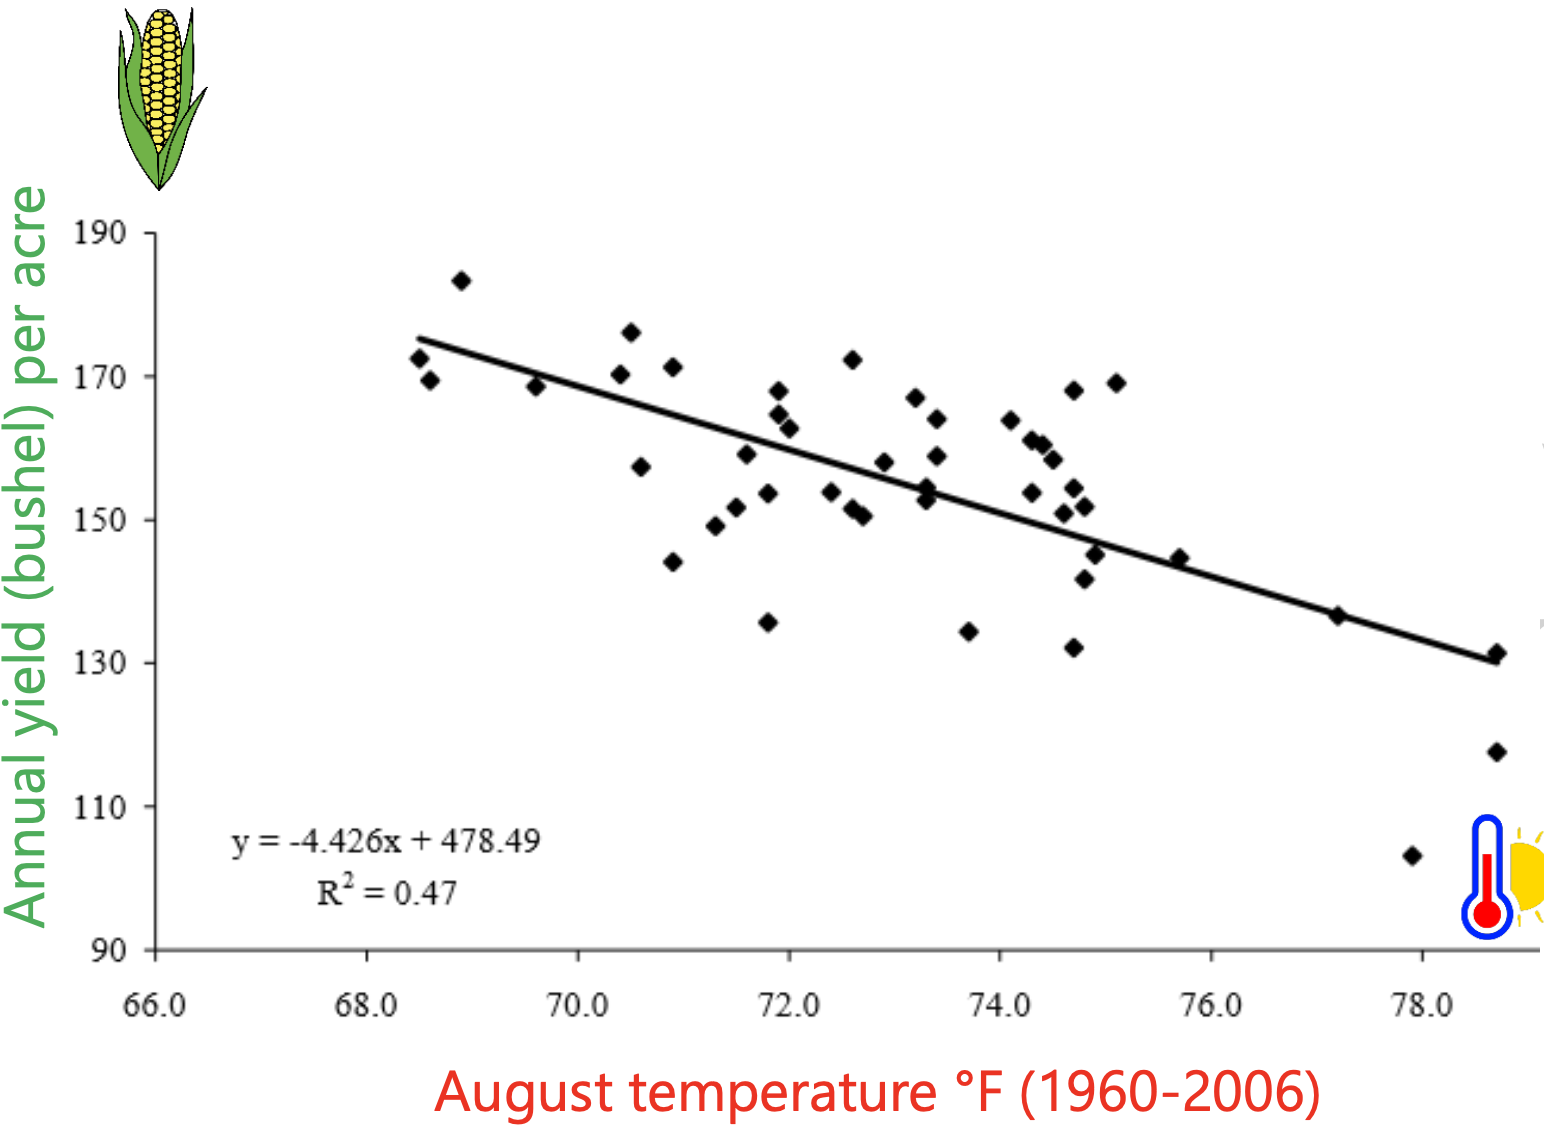
\includegraphics[width=3cm]{ep7.png}
{\tiny Illinois corn yield}
\end{figure}
\end{columns}
\end{frame}

\begin{frame}{Examples: Predicting values}
\begin{columns}
\column{0.75\textwidth}
\textbf{Problem}
\begin{itemize}
\item Online users' browsing and purchasing history
\item Predicting (in percentage terms) how likely the user is to click on an ad link / purchase an item
\end{itemize}
\vspace{6pt}
\textbf{Challenge}
\begin{itemize}
\item Input features of browsing and purchasing history are not numerical -- regression problem
\item Measurement of the similarity between items
\end{itemize}
\column{0.25\textwidth}
\begin{figure}
\centering
% Requires \usepackage{graphicx}
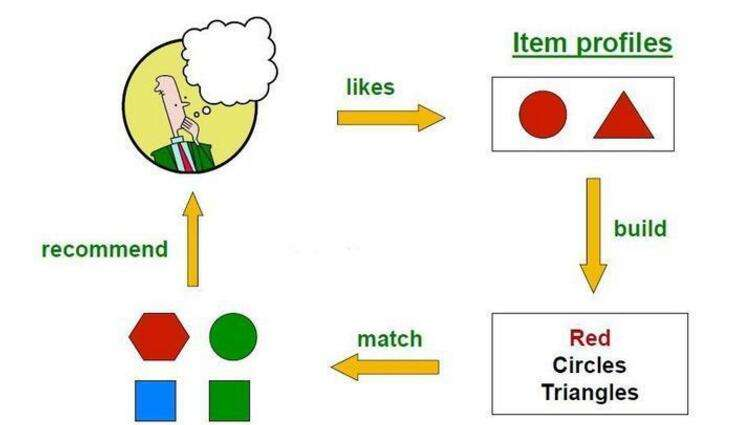
\includegraphics[width=3cm]{ep8.png}
{\tiny Intelligent recommendation}
\end{figure}
\end{columns}
\end{frame}

\begin{frame}{Correctness}
\textbf{Machine learning v.s. flipping a coin}
\begin{itemize}
\item Quantifying how well the learner is doing
\item Compare the level of success (eg. w.r.t. flipping a coin)
\end{itemize}
\vspace{6pt}
\textbf{Assessing correctness is difficult, due to, eg. unbalanced targets}
\begin{itemize}
\item Disease diagnoses: many diseases are pretty rare
\item Determining guilt: crime and criminals are relatively rare
\end{itemize}
\end{frame}

\begin{frame}{Correctness}
\textbf{Disease diagnoses: four issues to be considered}
\begin{itemize}
\item  How common is an illness (base rate)?
\item What is the cost of missing a diagnosis?
\item What is the cost of making a diagnosis (further costly and invasive testing / high level of anxiety)?
\item Doctors typically diagnose patients that come in the office (symptomatic).
\end{itemize}
\textbf{Determining guilt: different costs associated with failures}
\begin{itemize}
\item 99 criminals to go free v.s. 1 honest citizen to go to jail
\end{itemize}
\end{frame}

\begin{frame}{Correctness}
\begin{columns}
\column{0.75\textwidth}
\textbf{Two wrongs $\neq$ making a right}
\begin{itemize}
\item predicting rainfall in 2019 and 2020, based on data up to 2018 
\item over-predicting 500mm / per year in 2019
\item under-predicting 500mm / per year in 2020
\item plants receive 1.5 dose of water in 2019 and 0.5 dose of water in 2020
\item 0 harvest for TWO years!!!
\end{itemize}
\column{0.25\textwidth}
\begin{figure}
\centering
% Requires \usepackage{graphicx}

\includegraphics[width=3cm]{ep9.jpeg}
\end{figure}
\end{columns}
\end{frame}

\begin{frame}{Resource consumption}
\textbf{Time v.s. memory}
\begin{itemize}
\item How long does a computation take?
\item What is the maximum memory it needs?
\item Precomputing answers to common questions and store somewhere?
\item Example: Converting lengths from imperial to metric
$$
1 inch = 0.3048 m
$$
\end{itemize}
\vspace{6pt}
Different learning systems make different tradeoffs between what they remember about the data and how long they spend processing the data. 
\end{frame}

\begin{frame}{Building learning systems}
\textbf{We face}
\begin{itemize}
\item Learning problems in different domains, such as business, medicine and science
\item Different learning tasks
\item Different types of data
\item Different models relating input features to a target
\end{itemize}
\end{frame}

\begin{frame}{Building learning systems}
\begin{columns}
\column{0.75\textwidth}
\textbf{High-level steps}
\begin{itemize}
\item Develop an understanding of our task
\item Collect and understand our data
\item Prepare the data for modelling (Features? additional data?)
\item Build models of relationships in the data (Algorithm?)
\item Evaluate and compare one or more models
\item Tansition the model into a deployable system
\end{itemize}
\vspace{6pt}
\textbf{Process is not a straight line forward}
\begin{itemize}
\item Iterating and repeating the steps
\item Some steps may feed back to prior steps
\end{itemize}
\column{0.25\textwidth}
\begin{figure}
\centering
% Requires \usepackage{graphicx}
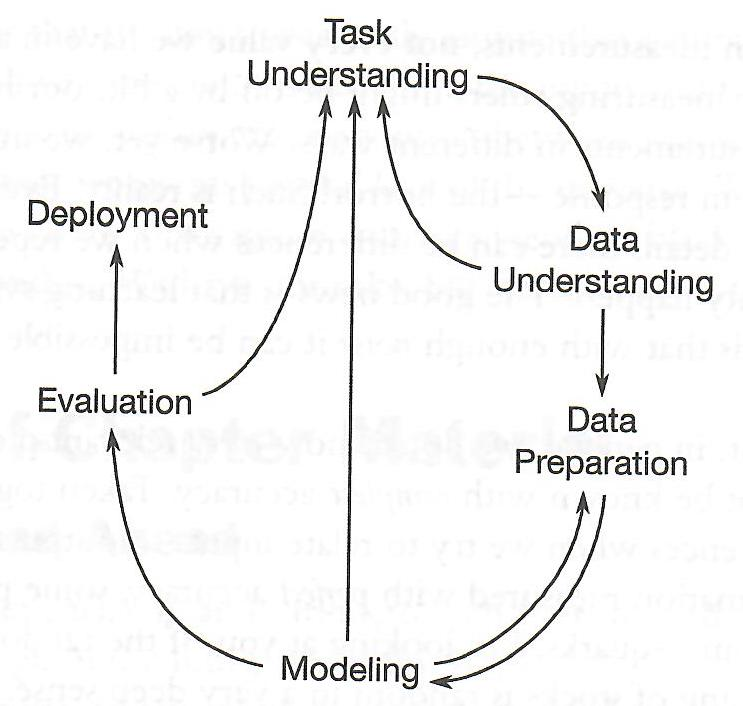
\includegraphics[width=3cm]{ep10.jpeg}
\end{figure}
\end{columns}
\end{frame}

\begin{frame}{Building learning systems}
\textbf{Low-level process (purpose of this course)}
\begin{itemize}
\item The task is abstracted
\item A pile of data gathered
\item Just make a learning system go!!!
\begin{itemize}
\item Finding usable examples
\item Applying different learning systems
\item Evaluating the results / Comparing alternatives
\item Implement the algorithm
\end{itemize}
\end{itemize}
\end{frame}

\begin{frame}{Reality of learning}
\begin{columns}
\column{0.75\textwidth}
\textbf{Noise}
\begin{itemize}
\item Irrelevant features: heart disease and sock colors
\item Measurement error
\end{itemize}
\vspace{3pt}
\textbf{Data size}
\begin{itemize}
\item The more the better? maybe not useful
\item A strong machine is helpful
\end{itemize}
\vspace{3pt}
\textbf{Missing feature}
\begin{itemize}
\item 3D objects that can give the same 2D shadow
\end{itemize}
\vspace{3pt}
Last caveat: we don't necessarily assume that nature operates the same way as our machine.;)))))
\column{0.25\textwidth}
\begin{figure}
\centering
% Requires \usepackage{graphicx}
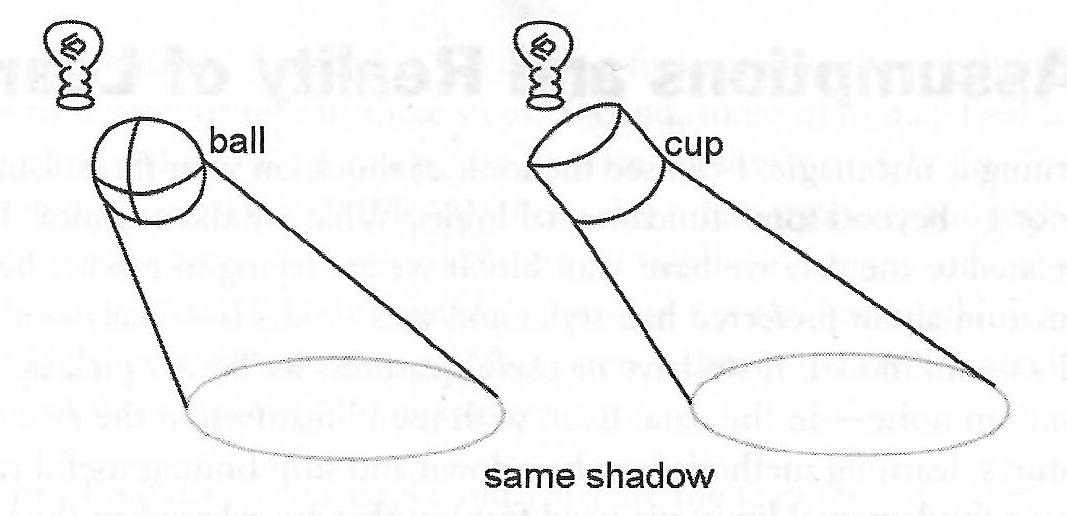
\includegraphics[width=3.2cm]{ep11.jpeg}
\end{figure}
\end{columns}
\end{frame}

\begin{frame}{Supervised learning}
\textbf{Catagory of machine learning}
\begin{itemize}
\item Supervised learning
\item Unsupervised learning
\item Semi-supervised learning
\item Reinforcement learning (Deep learning?)
\end{itemize}
\vspace{6pt}
\textbf{Basic elements}
\begin{itemize}
\item Input features -- training data
\item Learning system -- training systems - hypothesis 
\item Measurement of correctness -- evaluation criterion -- strategy
\item Algorithm
\end{itemize}
\end{frame}

\begin{frame}{Supervised learning}
\textbf{Mathematical settings}
\begin{itemize}
\item Example, instance $x_i$, $i= 1, 2, \ldots, N$
\item Feature vector 
$$
x_i = (x^{(1)}_i, x^{(2)}_i, \ldots, x^{(n)}_i)^{\rm T}
$$
\item Feature space $\{0, 1, \ldots, K_1\}\times\ldots\times \{0, 1, \ldots, K_{n_1}\}\times\mathbb{R}^{n_2}$
\item Training data
$$
T= \{(x_1, y_1), (x_2, y_2),\ldots,  (x_N, y_N)\}
$$
\item Output feature $y$
\begin{itemize}
\item classification problem, regression problem
\end{itemize}
\end{itemize}
\end{frame}

\begin{frame}{Supervised learning}
\textbf{Joint distribution of (X, Y)}
\begin{itemize}
\item The input features and output features are regarded as random variables
\item Subject to a joint distribution
\item P(X, Y) denotes either a distribution function or a density function
\item The leaning system does NOT know the joint distribution
\item Training data and testing data are i.i.d. samples from the joint distibution
\end{itemize}
\end{frame}

\begin{frame}{Supervised learning}
\textbf{Hypothesis space}
\begin{itemize}
\item Learning system aims to find a mapping from input to output feature
\item The collection of models forms a hypothesis space
\item The ways to formulate the mapping ("best" model)
\begin{itemize}
\item Conditional probability distribution (density) $P(Y|X)$
\item Decision function $Y=f(X)$
\end{itemize}
\end{itemize}
\end{frame}

\begin{frame}{Supervised learning}
\textbf{Formulation of the problem}
\begin{figure}
\centering
% Requires \usepackage{graphicx}
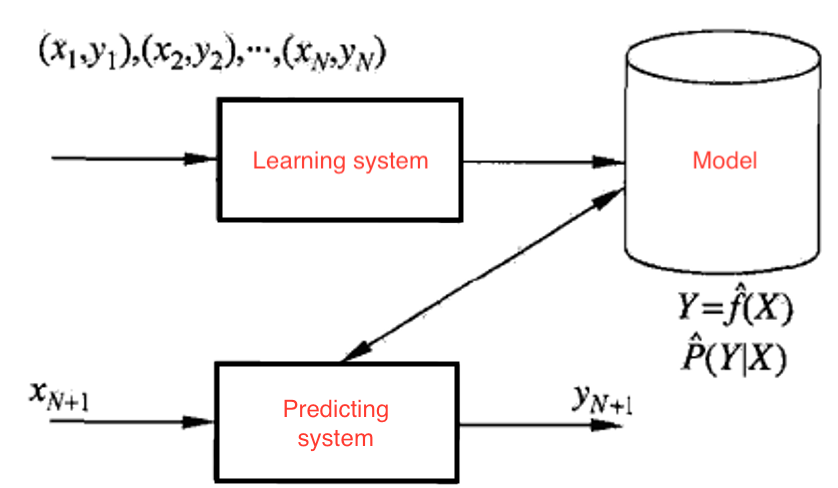
\includegraphics[width=5cm]{ep12.png}
\end{figure}
\begin{itemize}
\item 
$$
y_{N+1} = {\rm argmax}_{y_{N+1}}\widehat{P}(y_{N+1}|x_{N+1})
$$
\item 
$$
y_{N+1} = \widehat{f}(x_{N+1})
$$
\end{itemize}
\end{frame}

\begin{frame}{Unsupervised learning}
\textbf{Formulation of the problem}
\begin{figure}
\centering
% Requires \usepackage{graphicx}
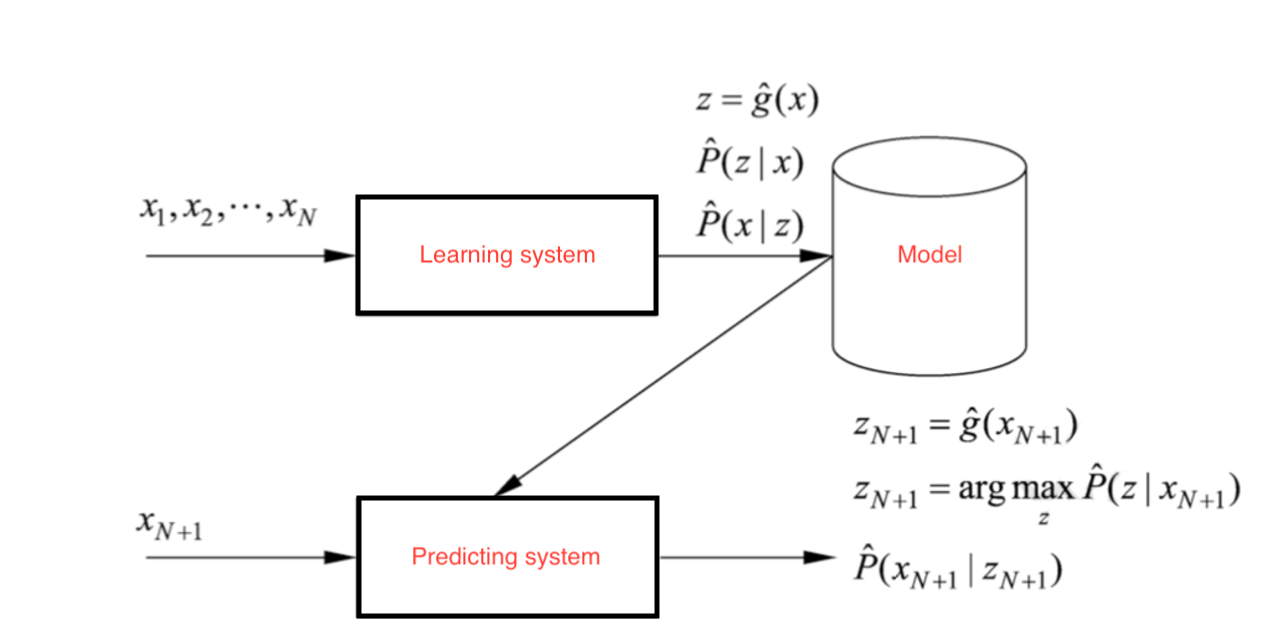
\includegraphics[width=5cm]{ep13.png}
\end{figure}
\begin{itemize}
\item Training data $$\{x_1, x_2, \ldots, x_N\}$$
\item Models
\begin{itemize}
\item Conditional probability distribution $P(z|x)$
\item Decision function $z = g(x)$
\end{itemize}
\end{itemize}
\end{frame}

\begin{frame}{Unsupervised learning}
\textbf{Example: SVM}
\begin{figure}
\centering
% Requires \usepackage{graphicx}
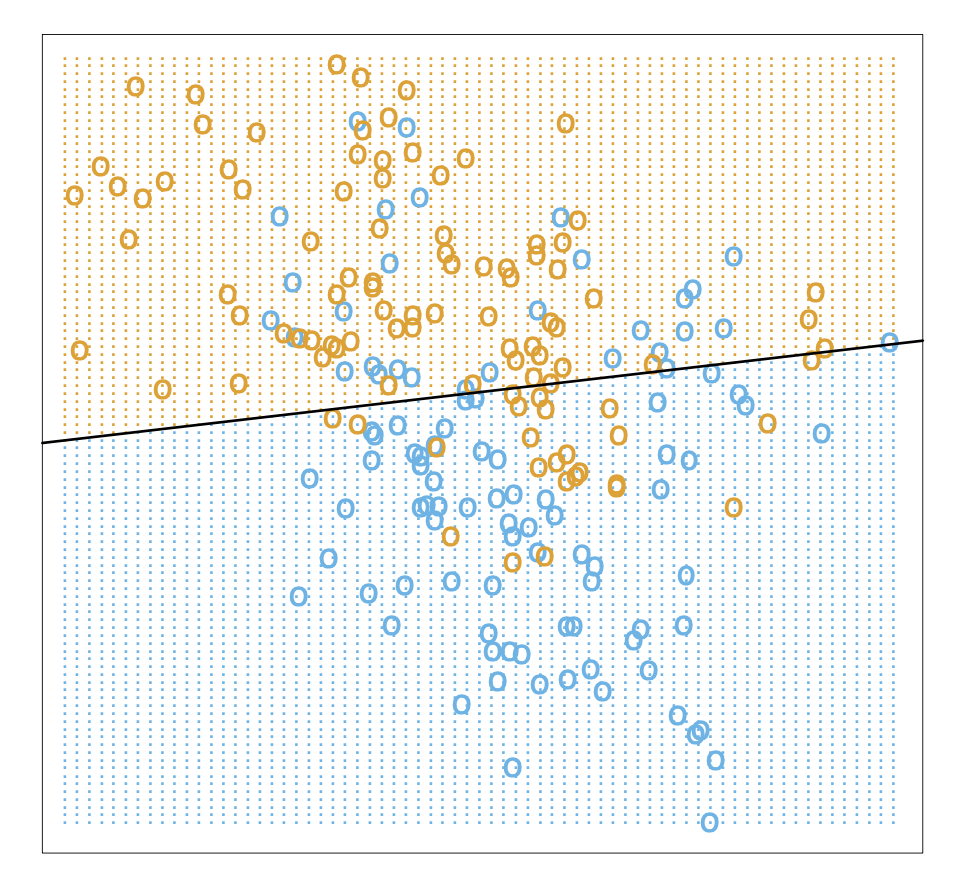
\includegraphics[width=5cm]{ep15.png}
\end{figure}
\end{frame}

\begin{frame}{Semi-supervised learning}
\textbf{Why?}
\begin{itemize}
\item A few of labelled data and  a large amount of unlabelled data
\item Labeled data produce considerable improvement in learning accuracy
\item Acquisition of unlabelled data is relatively inexpensive
\end{itemize}
\begin{figure}
\centering
% Requires \usepackage{graphicx}
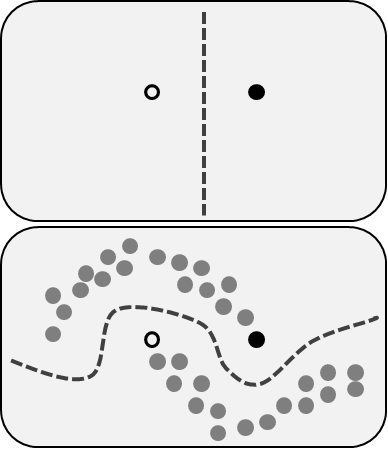
\includegraphics[width=2.5cm]{ep14.png}
\end{figure}
\end{frame} 

\begin{frame}{Reinforcement learning}
\begin{columns}
\column{0.75\textwidth}
\textbf{Formulation of the problem}
\begin{itemize}
\item Markov decision process with five elements $(S, A, P, r, \gamma)$
\item State space $S$, Action space $A$
\item Transition probability on states and actions
$$
P(s'|s, a)=P(s_{t+1} = s' | s_t = s, a_t = a)
$$
\item Reward function $r$: $$r(s, a) = E(r_{t+1}|s_t = s, a_t = a)$$
\item Discount factor $\gamma\in [0, 1]$
\end{itemize}
\column{0.25\textwidth}
\begin{figure}
\centering
% Requires \usepackage{graphicx}
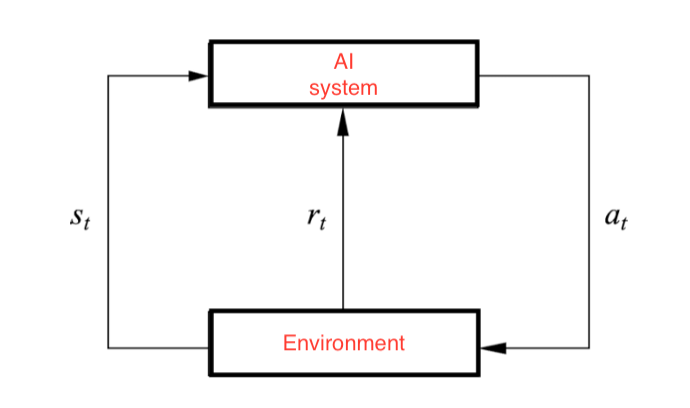
\includegraphics[width=3.2cm]{ep16.png}
\end{figure}
\end{columns}
\end{frame}

\begin{frame}{Reinforcement learning}
\textbf{Optimal decision}
\begin{itemize}
\item Optimal policy $\widehat{\pi}$: $\widehat{a}=\widehat{f}(s)$ or $\widehat{P}(a | s)$
\item Maximisation of the state value function
$$
v_\pi(s) = E_{\pi}[r_{t+1}+\gamma r_{t+2}+\ldots|s_t = s]
$$
and the action value function
$$
q_\pi(s, a) = E_{\pi}[r_{t+1}+\gamma r_{t+2}+\ldots|s_t = s, a_t = a]
$$
\item Learning the transition probability of the Markov process and the reward function
\item Learning the feedback of the environment  
\end{itemize}
\end{frame}

\begin{frame}{Evaluation criterion}
\textbf{For probability models $P(X, Y)$, $P(Y|X)$}
\begin{itemize}
\item Maximum Likelihood Estimate
\item Bayesian estimate (on the posterior probability)
\end{itemize}
\begin{figure}
\centering
% Requires \usepackage{graphicx}
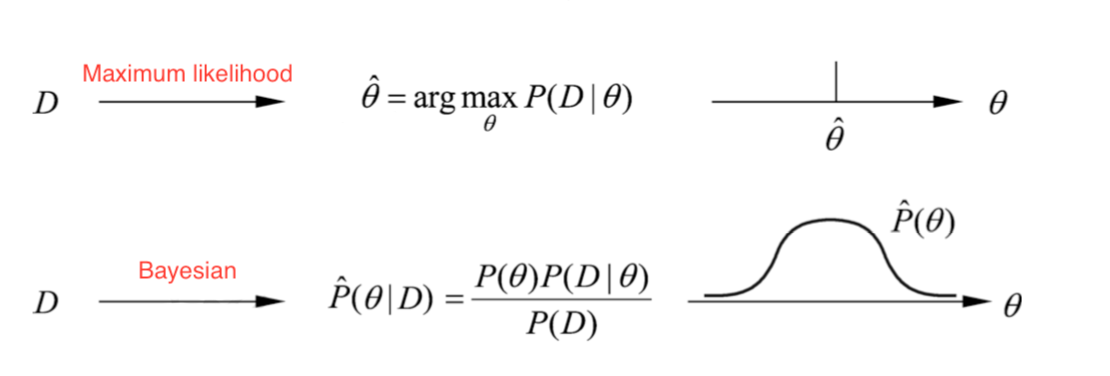
\includegraphics[width=8cm]{ep17.png}
\end{figure}
\end{frame}

\begin{frame}{Evaluation criterion}
\textbf{Prediction with probability models}
\begin{itemize}
\item With maximum likelihood estimator $\widehat{\theta}$
$$
\widehat{y}_{MLE} = E_{\widehat{\theta}}(y|x)
$$
\item With Bayesian posterior probability ${P}(\theta | D)$
$$
\widehat{y}_{Bayesian} = \int \int y P(y|x, \theta, D) P(\theta | D) d\theta dy
$$
\end{itemize}
\end{frame}

\begin{frame}{Evaluation criterion}
\textbf{For decision function $f(X)$}
\begin{itemize}
\item Loss function: measurement of the prediction quality of a particular prediction
\item Risk function: measurement of the prediction quality in average
\item $0-1$ loss function
$$
L(Y, f(X)) = 1,\ {\rm if}\ Y\neq f(X); L(Y, f(X)) = 0,\ {\rm if}\ Y= f(X)
$$
\item Quadratic loss function
$$
L(Y, f(X)) = (Y-f(X))^2
$$
\end{itemize}
\end{frame}

\begin{frame}{Evaluation criterion}
\textbf{For decision function $f(X)$}
\begin{itemize}
\item Absolute loss function
$$
L(Y, f(X)) = |Y-f(X)|
$$
\end{itemize}
For probability model, similarly loss function can be defined for measuring the "distance" between two probability: the related entropy or logarithmic loss function.
\end{frame}

\begin{frame}{Evaluation criterion}
\textbf{Strategy}
\begin{itemize}
\item Minimisation of the risk function (the expectation of the loss function)
$$
R_{exp}(f) = E_{P}[L(Y, f(X))]
$$
\item $P$ is unknown!!!
\item Instead, empirical risk is a "nice" estimator for the risk function (proof is very very very hard)
$$
R_{emp}(f) = \frac{1}{N}\sum^N_{i=1}L(y_i, f(x_i))
$$
\end{itemize}
\end{frame}

\begin{frame}{Evaluation criterion}
\textbf{Strategy}
\begin{itemize}
\item Determining of the "best" model $\Longleftrightarrow$ minimisation of the empirical risk
$$
R_{emp}(f) \Longrightarrow {\rm min}
$$
\item The end of story??? NO!!!
\item Small example size $\Longrightarrow$ overfitting
\end{itemize}
\begin{figure}
\centering
% Requires \usepackage{graphicx}
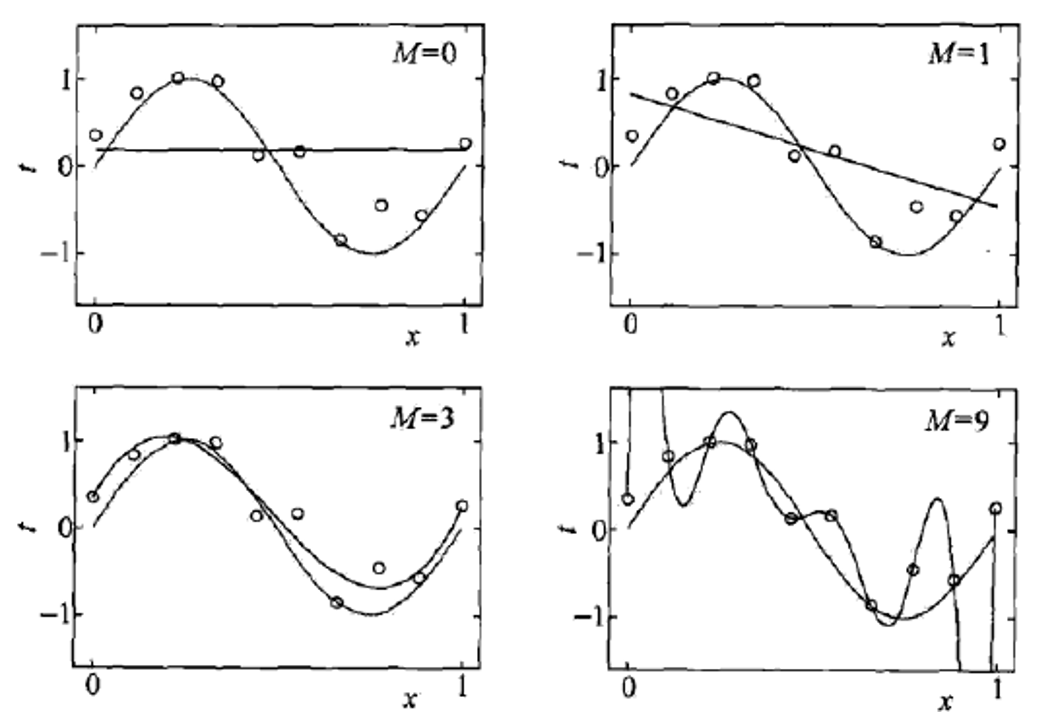
\includegraphics[width=4cm]{ep18.png}
\end{figure}
\end{frame}

\begin{frame}{Evaluation criterion}
\textbf{Is overfitting evitable?}
\begin{itemize}
\item Penalisation on the complexity (regularization)
$$
\min_{f\in \mathcal{F}} \frac{1}{N} \sum^N_{i=1} L(y_i, f(x_i)) + \lambda J(f)
$$
\item Examples from linear regression
$$
\min_w L(w) = \frac{1}{N} \sum^N_{i=1} (f(x_i; w) - y_i)^2 +\frac{\lambda}{2}||w||_2\ {\rm (RIDGE)}
$$
or 
$$
\min_w L(w) = \frac{1}{N} \sum^N_{i=1} (f(x_i; w) - y_i)^2 +\frac{\lambda}{2}||w||_1\ {\rm (LASSO)}
$$
\end{itemize}
\end{frame}

\begin{frame}{Evaluation criterion}
\textbf{Is overfitting evitable?}
\begin{itemize}
\item Cross-validation
\begin{itemize}
\item Simple cross-validation: training data + test data
\item Leave-one-out cross-validation
\item $k$-fold cross-validation
\end{itemize}
\end{itemize}
\begin{figure}
\centering
% Requires \usepackage{graphicx}
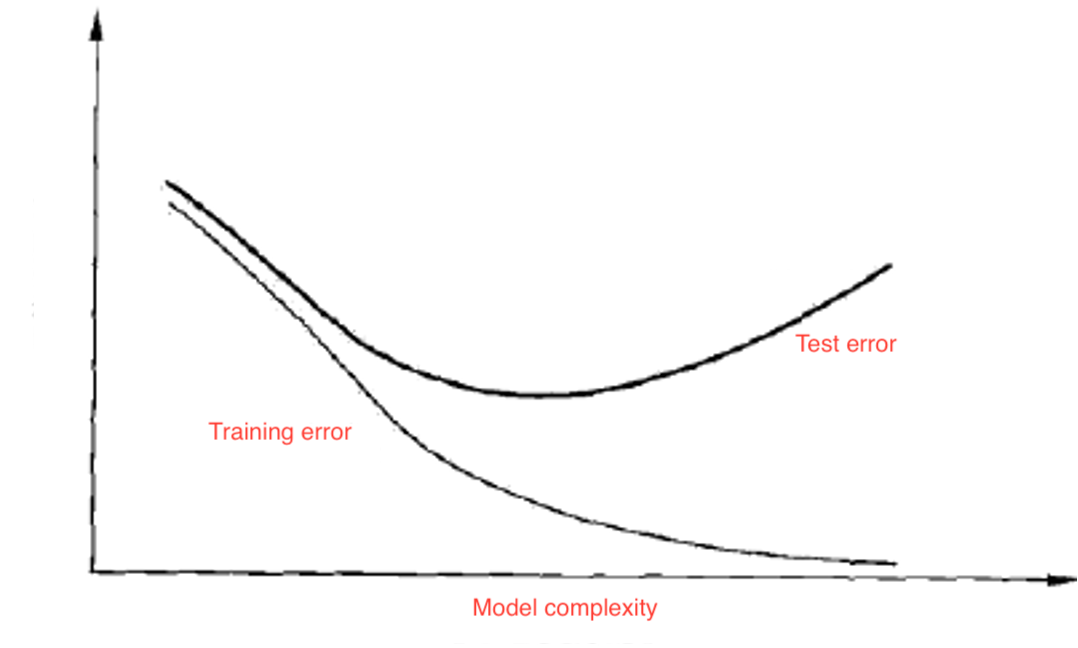
\includegraphics[width=5.4cm]{ep19.png}
\end{figure}
\end{frame}


\begin{frame}{}
\begin{center}
    \textbf{谢谢!}\\
    \textbf{Merci!}\\
    \textbf{Thanks!}
\end{center}
\end{frame}


\end{document}

